% Chapter Template

\chapter{Localization System Overview} % Main chapter title

\label{Chapter3} % Change X to a consecutive number; for referencing this chapter elsewhere, use \ref{ChapterX}
One of the key contributions of this work is the server-based localization architecture. In this chapter, we present our concrete system design. We provide an overview of the different physical components in the first part, following a second part where we introduce the components of the localization algorithm. 

%----------------------------------------------------------------------------------------
%	SECTION 1
%----------------------------------------------------------------------------------------

\section{Localization System Architecture}
Our proposed localization system consists of various components, such as a localization server, a target device, several UWB anchor nodes and WiFi access points. An overview of all these components can be seen in Figure \ref{fig:system_components}.\\
\begin{figure}[th]
\centering
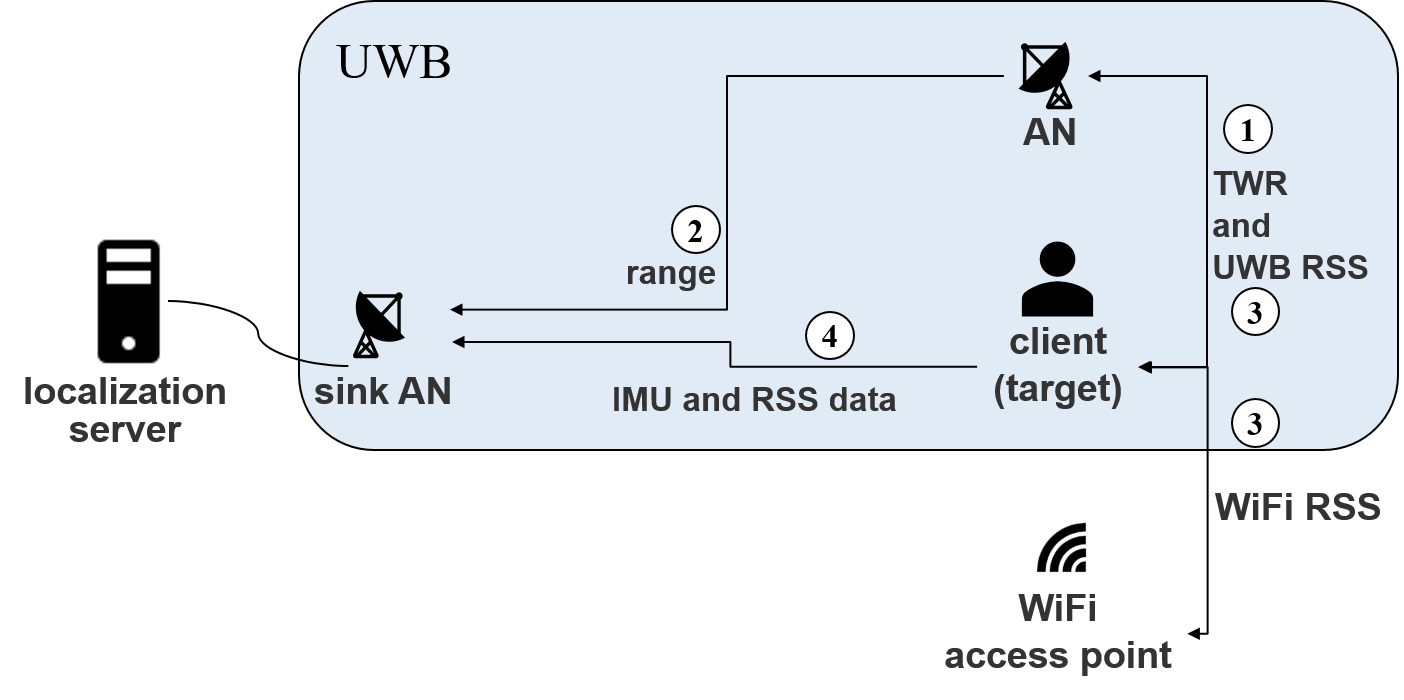
\includegraphics[width=1.0\textwidth]{Figures/system_components_numbers}
\decoRule
\caption[System Architecture]{Overview of the components in our localization system.}
\label{fig:system_components}
\end{figure}

\noindent\hspace*{5mm}%
On the localization server, most of the computational workload is handled. The localization algorithm runs on the server. It periodically requests input data from the other system elements and processes the data as soon as it arrives. The server updates the system state (e.g. particle positions, velocity) and estimates the position in every timestep. Additionally, a graphical illustration of the real-time position on the floormap is available on the server side. \\
\noindent\hspace*{5mm}%
The client is the target device that is localized. It is equipped with different IMU sensors, at least with a 3D accelerometer and a 3D magnetometer. With the sensor readings, the client performs a computation of the heading direction and the change in velocity. With the equipped WiFi module and the UWB transmitter, it collects RSS data of all WiFi access points and UWB anchor nodes in range. The heading direction, velocity change, and RSS fingerprint are transmitted from the client to the localization server.\\
\noindent\hspace*{5mm}%
Ultra-wideband anchor nodes are distributed over the area of interest to cover it homogeneously. One anchor node is specified as a sink AN, it is connected to the localization server with a wired Ethernet connection. The sink AN ensures the communication via UWB to the other ANs and the client device. It receives IMU and RSS data from the client and forwards it to the server. When triggered from the sink AN, the other anchor nodes perform two-way ranging to the TAG and forward the result via sink AN to the server.\\
\noindent\hspace*{5mm}%
Also the WiFi access points are spread over the area of interest. They fulfill only one purpose: They emit Wi-Fi radio signals that are detected by the client in order to measure the received signal strength.\\
\noindent\hspace*{5mm}%
The flow of messages in this architecture is indicated with arrows numbered from 1 to 4 in Figure \ref{fig:system_components}. The explanation of the numbers is:\\
\begin{enumerate}
\item The ANs perform the Two Way Ranging by sending a request to the client. 
\item The ANs forward the range measurement to the localization server.
\item The client communicates with the ANs and the WiFi access points to measure the signal strength.
\item The obtained RSS values are merged into a message together with measured sensor data. This message is transmitted back to the server.
\end{enumerate}


%----------------------------------------------------------------------------------------
%	SECTION 2
%----------------------------------------------------------------------------------------

\section{Localization Algorithm}
The particle filter localization algorithm consists of several tasks relying on different data inputs. An overview of the particle filter and its fused information is illustrated in Figure \ref{fig:localization_algorithm}. The four used data types are IMU sensor data, floorplan information, range estimations and RSS fingerprints.\\
\begin{figure}[th]
\centering
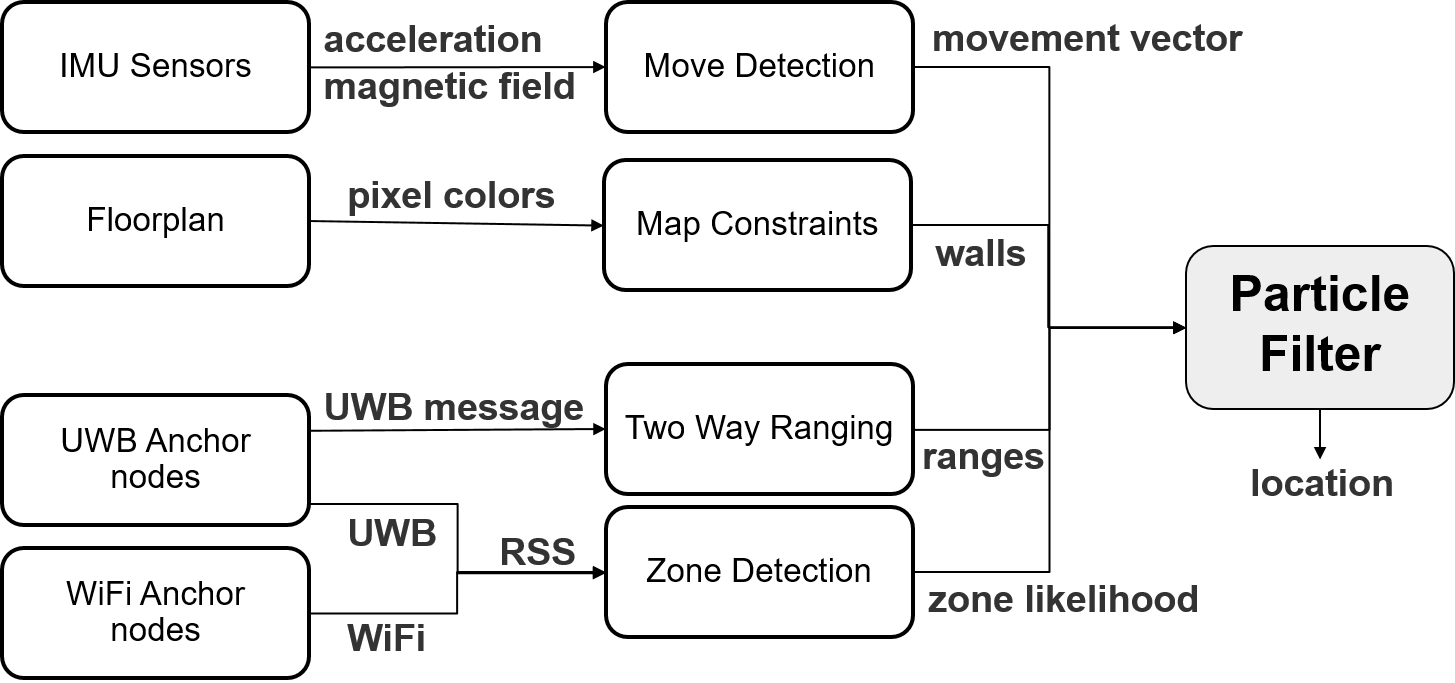
\includegraphics[width=1.0\textwidth]{Figures/localization_algorithm}
\decoRule
\caption[Localization Algorithm]{Overview of the localization algorithm components.}
\label{fig:localization_algorithm}
\end{figure}

\noindent\hspace*{5mm}%
The IMUs are measuring acceleration and magnetic field energy to obtain stride length and heading direction. In the movement detection, the stride length and the heading direction are converted to a movement vector, containing X and Y Cartesian coordinates in the buildings coordinate system.\\
\noindent\hspace*{5mm}%
Floorplan information is preprocessed from a given floorplan image. Based on the given information, a map of allowed and not allowed positions is generated, in order to quickly check whether a given particle position is allowed or not.\\
\noindent\hspace*{5mm}%  
Ranging information is obtained by two way ranging to every anchor node. The anchor node positions are preliminarily stored in the particle filter, such that it is sufficient to process a tupel (AN, range) of anchor node identifier and range measurement.\\
\noindent\hspace*{5mm}%  
The zone detection is fed with UWB and WiFi received signal strength data. Observing the concrete fingerprint of RSS data, for each zone a dedicated probability for being in that zone is computed.\\
\noindent\hspace*{5mm}%  
In the particle filter, the different inputs are fused. The prediction phase takes only the floorplan constraints into account, whereas for the observation phase the other three inputs - range estimation, zone likelihood and movement vector - are used to determine the weight of a certain particle.\\
\noindent\hspace*{5mm}%
Given the position and the weight of each particle, the system calculates the weighted sum over the particle positions to obtain the localization estimation. The construction of the weight for each particle ensures that more likely positions have a bigger impact on the position estimation than more unlikely positions.